\part{光线追踪}

\chapter{阴影}

在着色这一部分, 我们介绍了如何对各个物体计算对应像素的颜色. 然而, 我们的计算对于每个模型来说都是独立的, 并没有考虑光的遮挡关系. 因此我们在这里说明在光栅化的情况下, 如何计算阴影. 

\section{Shadow Mapping}
\textbf{Shadow Mapping}是一种图像空间的算法. 在计算阴影的时候我们不需要知道场景的几何信息. Shadow Mapping的方法只适用于在点光源下计算硬阴影.
硬阴影指的是一个点是否在阴影内是确定的, 它不是在阴影内就在阴影外; 只有点光源才可以产生这种情况. 软阴影指的是阴影是有过渡的, 一个点可以接收到部分光线; 当不忽略光源大小的时候, 就会产生这种情况.
可以接收到部分光线的区域一般称为半影. 

一个点是否在阴影中取决于光源和摄像机是不是都可以看到这个点. 如果都可以看到这个点, 那么说明这个点不在阴影里. 因此我们使用如下方式进行计算: 
\begin{enumerate}
	\item 从光源位置看向场景, 做出深度图; 
	\item 从摄像机位置看向场景, 对于每一个看到的点, 计算到光源的距离, 并且得到光源深度图上对应像素点的距离进行比较. 如果距离一样, 那么说明这个点不在阴影中, 反之, 这个点在阴影中. 
\end{enumerate}

这样的算法有两个问题: 
\begin{enumerate}
	\item 距离是一个浮点数, 不容易进行比较. 需要引入一定的宽容度. 这是数值精度的问题, 不能从本质解决问题; 
	\item 阴影的质量和光源深度图的分辨率有关. 如果光源深度图太小, 但是摄像机分辨率大就容易出现走样问题; 
	\item 这个方法只适合硬阴影, 不适合软阴影. 
\end{enumerate}

因此, 我们需要引入光线追踪的方法来解决光栅化Shadow Mapping中可能出现的问题. 

\begin{figure}[H]
	\centering
	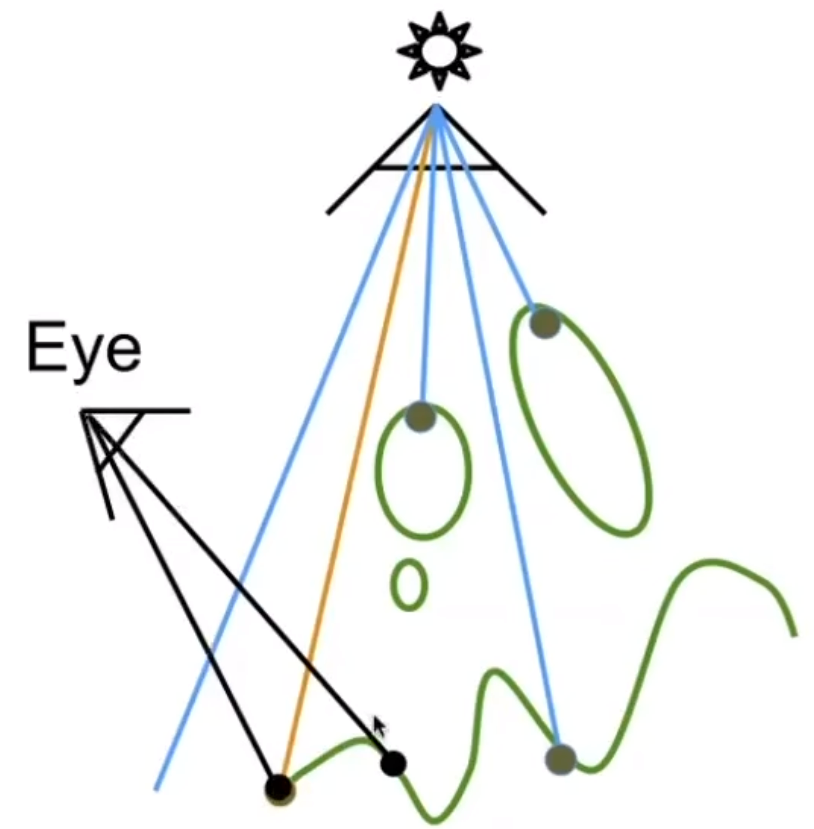
\includegraphics[scale=.5]{ShadowMapping_1.png}
	\caption{相机视角的深度与点光源视角的深度一致, 可见}
	\label{fig:ShadowMapping_1}
\end{figure}

\begin{figure}[H]
	\centering
	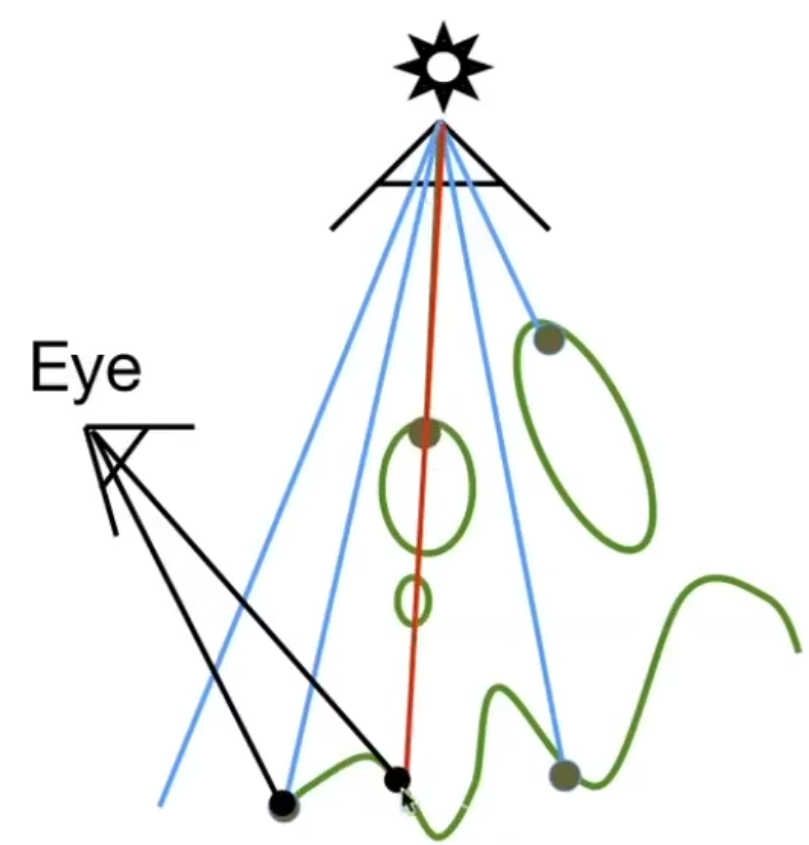
\includegraphics[scale=.5]{ShadowMapping_2.png}
	\caption{相机视角的深度与点光源视角的深度不一致, 不可见}
	\label{fig:ShadowMapping_2}
\end{figure}





\chapter{光线追踪}

\section{基础知识}

我们引入光线追踪, 主要是为了解决光栅化中没有解决的一些问题: 
\begin{enumerate}
	\item 全局的光照效果不好表示; 
	\item 软阴影效果的产生; 
	\item 光泽反射 (Glossy reflection, 一种类似于镜面反射的情况, 但是没有镜面光滑的表面产生的情况) 会让光线在场景中多次反射; 
	\item 间接光照, 在漫反射场景中, 有些光线在到达眼睛前反射不止一次. 
\end{enumerate}

光栅化是一种比较快速, 近似的一种渲染方式, 用于实时渲染; 光线追踪是比较准确但是比较慢的渲染方式, 用于离线渲染. 

\subsection{基本光线追踪方法}

\subsubsection{光线的定义}

我们假设光线有以下三个性质: 
\begin{enumerate}
	\item 光沿直线传播; 
	\item 光线和光线不会发生碰撞的交叉; 
	\item 光线从光源射入人眼中. 
\end{enumerate}
因此我们可以利用光的可逆性 (Reciprocity) 进行光线追踪. 光线追踪是指我们从摄像机沿着每一个像素点的连线射出光线, 追踪光线的路径. 

\subsubsection{光线追踪的假设}
我们认为眼睛是一个点, 光源均为点光源. 我们从眼睛沿着像素点画一条光线, 如果光线和物体有接触, 我们将交点和光源进行连线, 如果可以连接到光源, 那我们认为这一点被照亮, 可以计算着色. 

\subsection{Whitted-Style光线追踪}
从眼睛沿着像素连接一条光线, 我们认为光线在传播的过程中发生反射和折射现象. 假设反射是完美的镜面反射. 当我们将所有的反射 (折射) 点和光源连接起来. 如果这一点可以被光源照亮, 那么我们认为这一点的着色应当叠加在这个像素上. 对于光线我们认为存在能量的消逝, 不会一直反射. 

\begin{figure}[H]
	\centering
	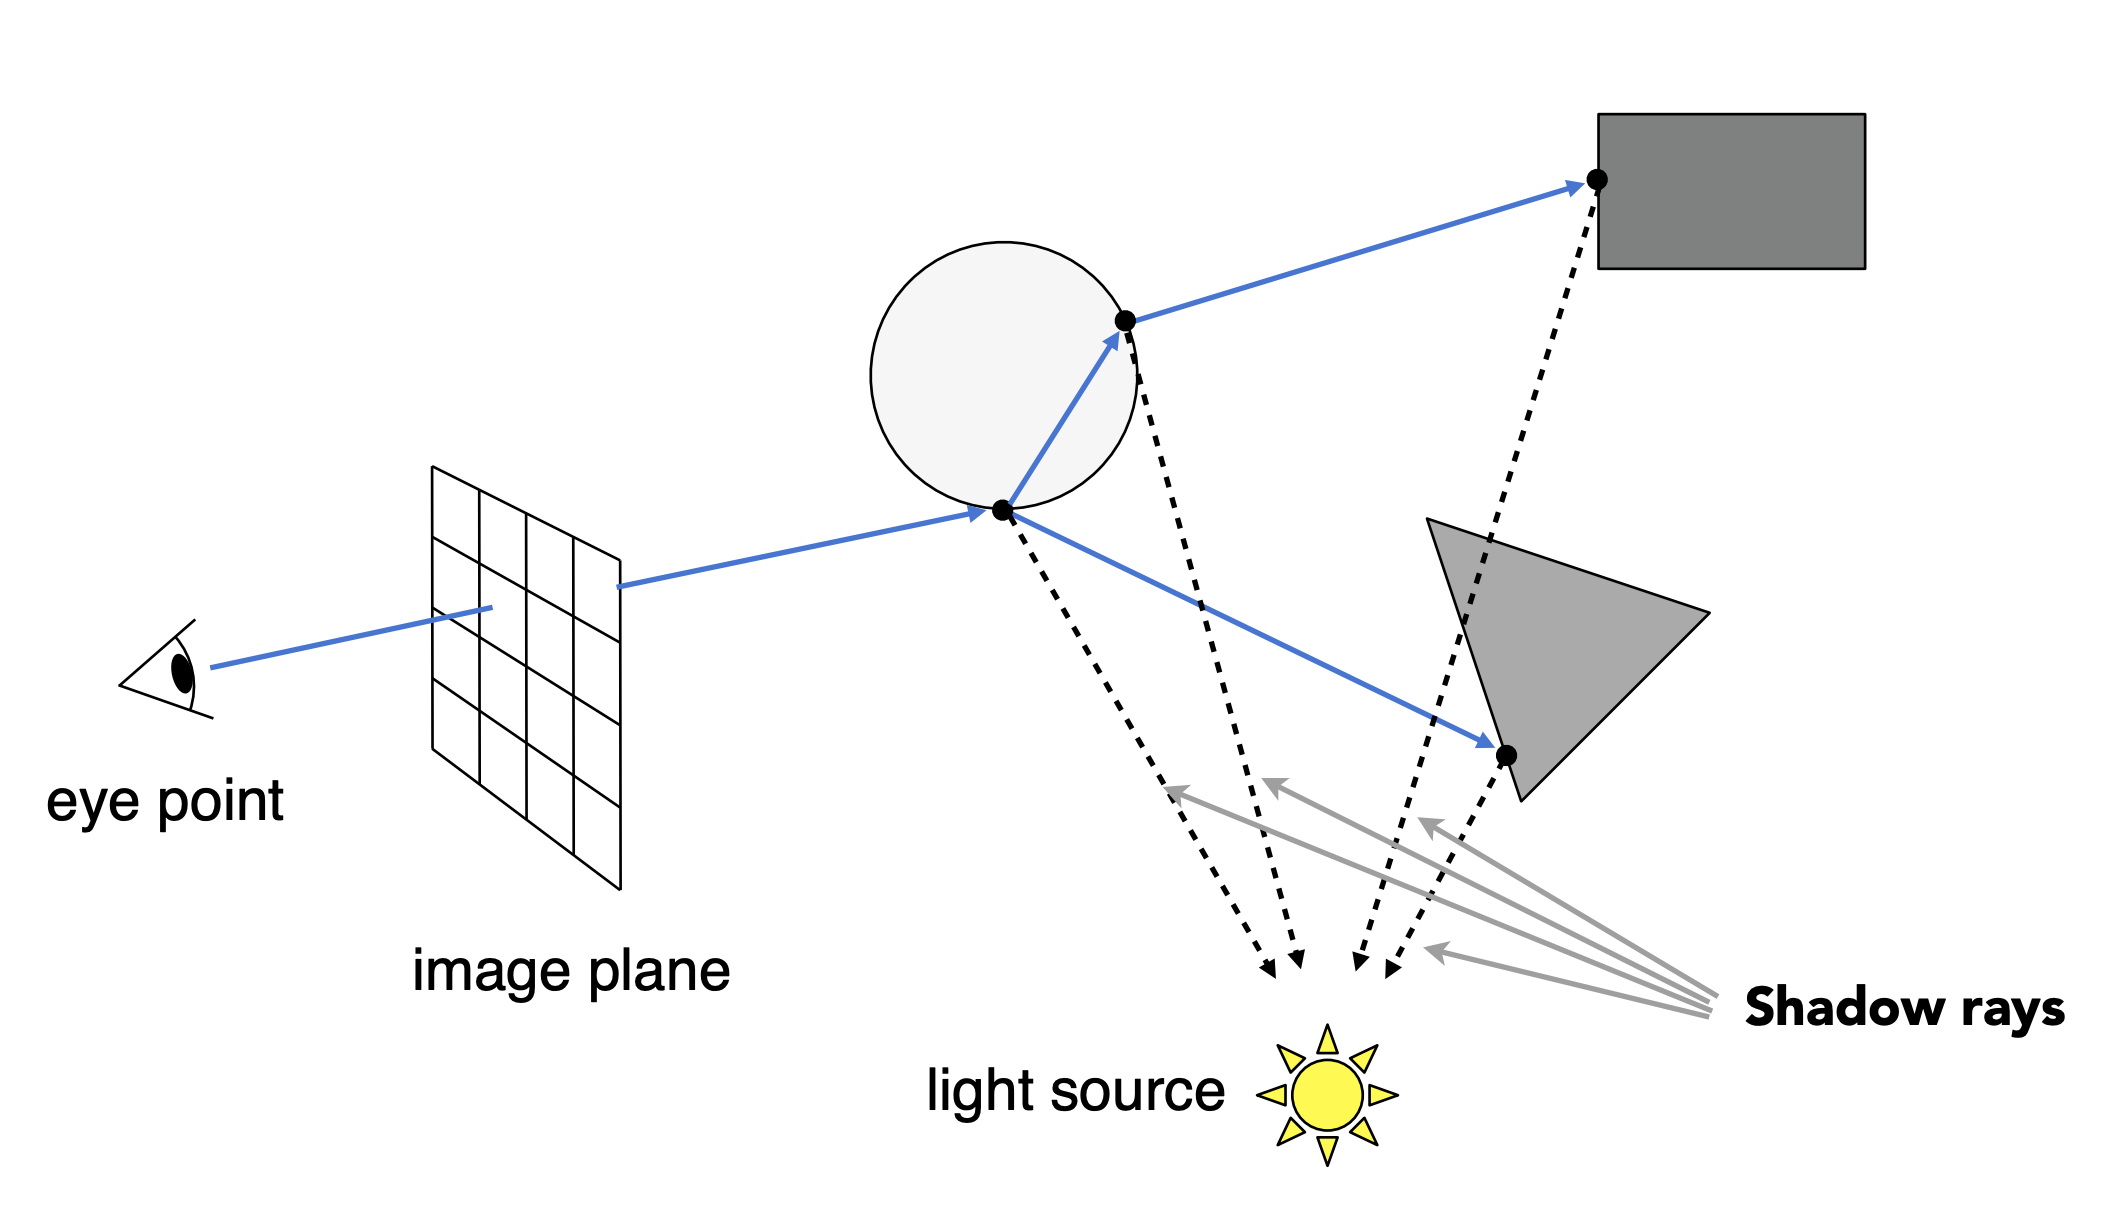
\includegraphics[scale=.25]{guangxianzhuizong.png}
	\caption{Whitted-Style光线追踪示意图}
	\label{fig:gxzz}
\end{figure}
眼睛和像素直接连接起来的光线称为primary ray, 发生反射和折射后形成的光线称为secondary ray, 反射点和光源的连线称为shadow ray. 

\subsection{光线-表面交点}
对于光线追踪而言, 最重要的就是求出光线和物体的交点. 首先我们对光线进行定义. 我们假设光线的起点为$o$, 光线的方向是单位向量$d$, 那么光线就可以定义为$o+td$. 

\subsubsection{光线和球面的交点}

我们首先计算光线和球面的交点作为引入. 光线我们可以表示为: 
\begin{equation}
	r(t)=o+td, 0\le t \le \infty
\end{equation}

对于球面, 我们可以表示为: 
\begin{equation}
	(p-c)^2-R^2=0
\end{equation}其中, $c$是球心, $p$是任意一点. 如果$p$是光线和球面的交点, 那么这个点可以同时满足上面两个函数. 因此, 我们将光线公式代入到球面公式上就可以得到它们的交点: 
\begin{equation}
	(o+td-c)^2-R^2=0
\end{equation}
这是一个二元一次方程组, 使用求根公式就可以得到结果. 我们讨论求根公式中$\triangle$值. 如果$\triangle < 0$, 那么光线和球体没有交点; 如果$\triangle = 0$, 光线和球体相切; 如果$\triangle > 0$, 那么光线穿过球体, 有两个交点. 

\subsubsection{光线和隐式函数面的交点}

光线我们可以表示为: 
\begin{equation}
	r(t)=o+td, 0\le t \le \infty
\end{equation}

对于任意一个隐式函数面, 我们定义为: 
\begin{equation}
	f(p)=0
\end{equation}

我们可以直接把光线公式代入隐式函数中求出结果: 
\begin{equation}
	f(o+td)=0
\end{equation}

\subsubsection{光线和显式三角形面的交点}
我们可以通过求交点的方式判断一个点是否在封闭曲面的内部还是外部. 任何一个点发出一条光线, 如果交点个数为奇数, 那么这个点一定在封闭曲面内部; 如果有偶数个点, 那么这个点一定在封闭曲面的外部. 

我们求一条光线和显式三角形面的交点可以分为两步: 
\begin{enumerate}
	\item 求出光线和三角形面所在平面的交点; 
	\item 判断这个点是否在三角形内 (之前的课程中已经介绍了判断的方法) . 
\end{enumerate}

我们使用法线$N$和平面上的任意一个点$p‘$来定义一个平面: 
\begin{equation}
	(p-p')\cdot N = 0
\end{equation}
其中$p'$是平面上任意一点, 满足条件的$p$都在这个平面上. 我们令$p=o+td$就可以求出光线和这个平面的交点, 
\begin{equation}
	(p-p')\cdot N = (o+td-p')\cdot N = 0
\end{equation}
可以求出: 
\begin{equation}
	t = \frac{(p'-o)\cdot N}{d\cdot N}, 0\le t \le \infty
\end{equation}

我们可以通过另一种算法直接求出一条光线和一个显式三角形面是否有交点. 任何一个显式的三角形内部的一个点都可以写成三个顶点的线性组合. 因此我们可以得到: 
\begin{equation}
	o+td=(1-b_1-b_2)P_0+b_1P_1+b_2P_2
\end{equation}使用克莱姆法则可以得到: 
\begin{equation}
	\begin{bmatrix}
		t\\ 
		b_1\\ 
		b_2
	\end{bmatrix}=\frac{1}{S_1\cdot E_1}\begin{bmatrix}
		S_2\cdot E_2\\ 
		S_1\cdot E\\ 
		S_2\cdot D
	\end{bmatrix}
\end{equation}其中, $E_1=P_1-P_0,E_2=P_2-P_0,S=O-P_0,S_1=D\times E_2, S_2=S\times E_1$.最后我们只需要判断这个解是否合理即可, 只要求解出的三个量都是非负的, 那么光线和显式三角形面有一个交点. 

\section{光线追踪加速}
传统的计算方法所需要的计算消耗量非常大, 因此我们需要通过一些方式加速计算. 
\subsection{包围体积}
\textbf{包围体积 (Bounding Volume) }使用一个简单的立方体包围复杂的模型. 如果光线连包围盒都碰不到, 那么光线一定不能碰到里面的物体. 
我们常用的包围盒是\textbf{轴对其包围盒 (Axis-Aligned Bounding Box,  AABB) }, 包围盒的长宽高和坐标轴都是平行的. 我们认为, 包围体积是三组成对平面的交集. 为了计算光线和包围盒的相交情况, 我们在二维情况下进行简化计算: 
\begin{figure}[H]
	\centering
	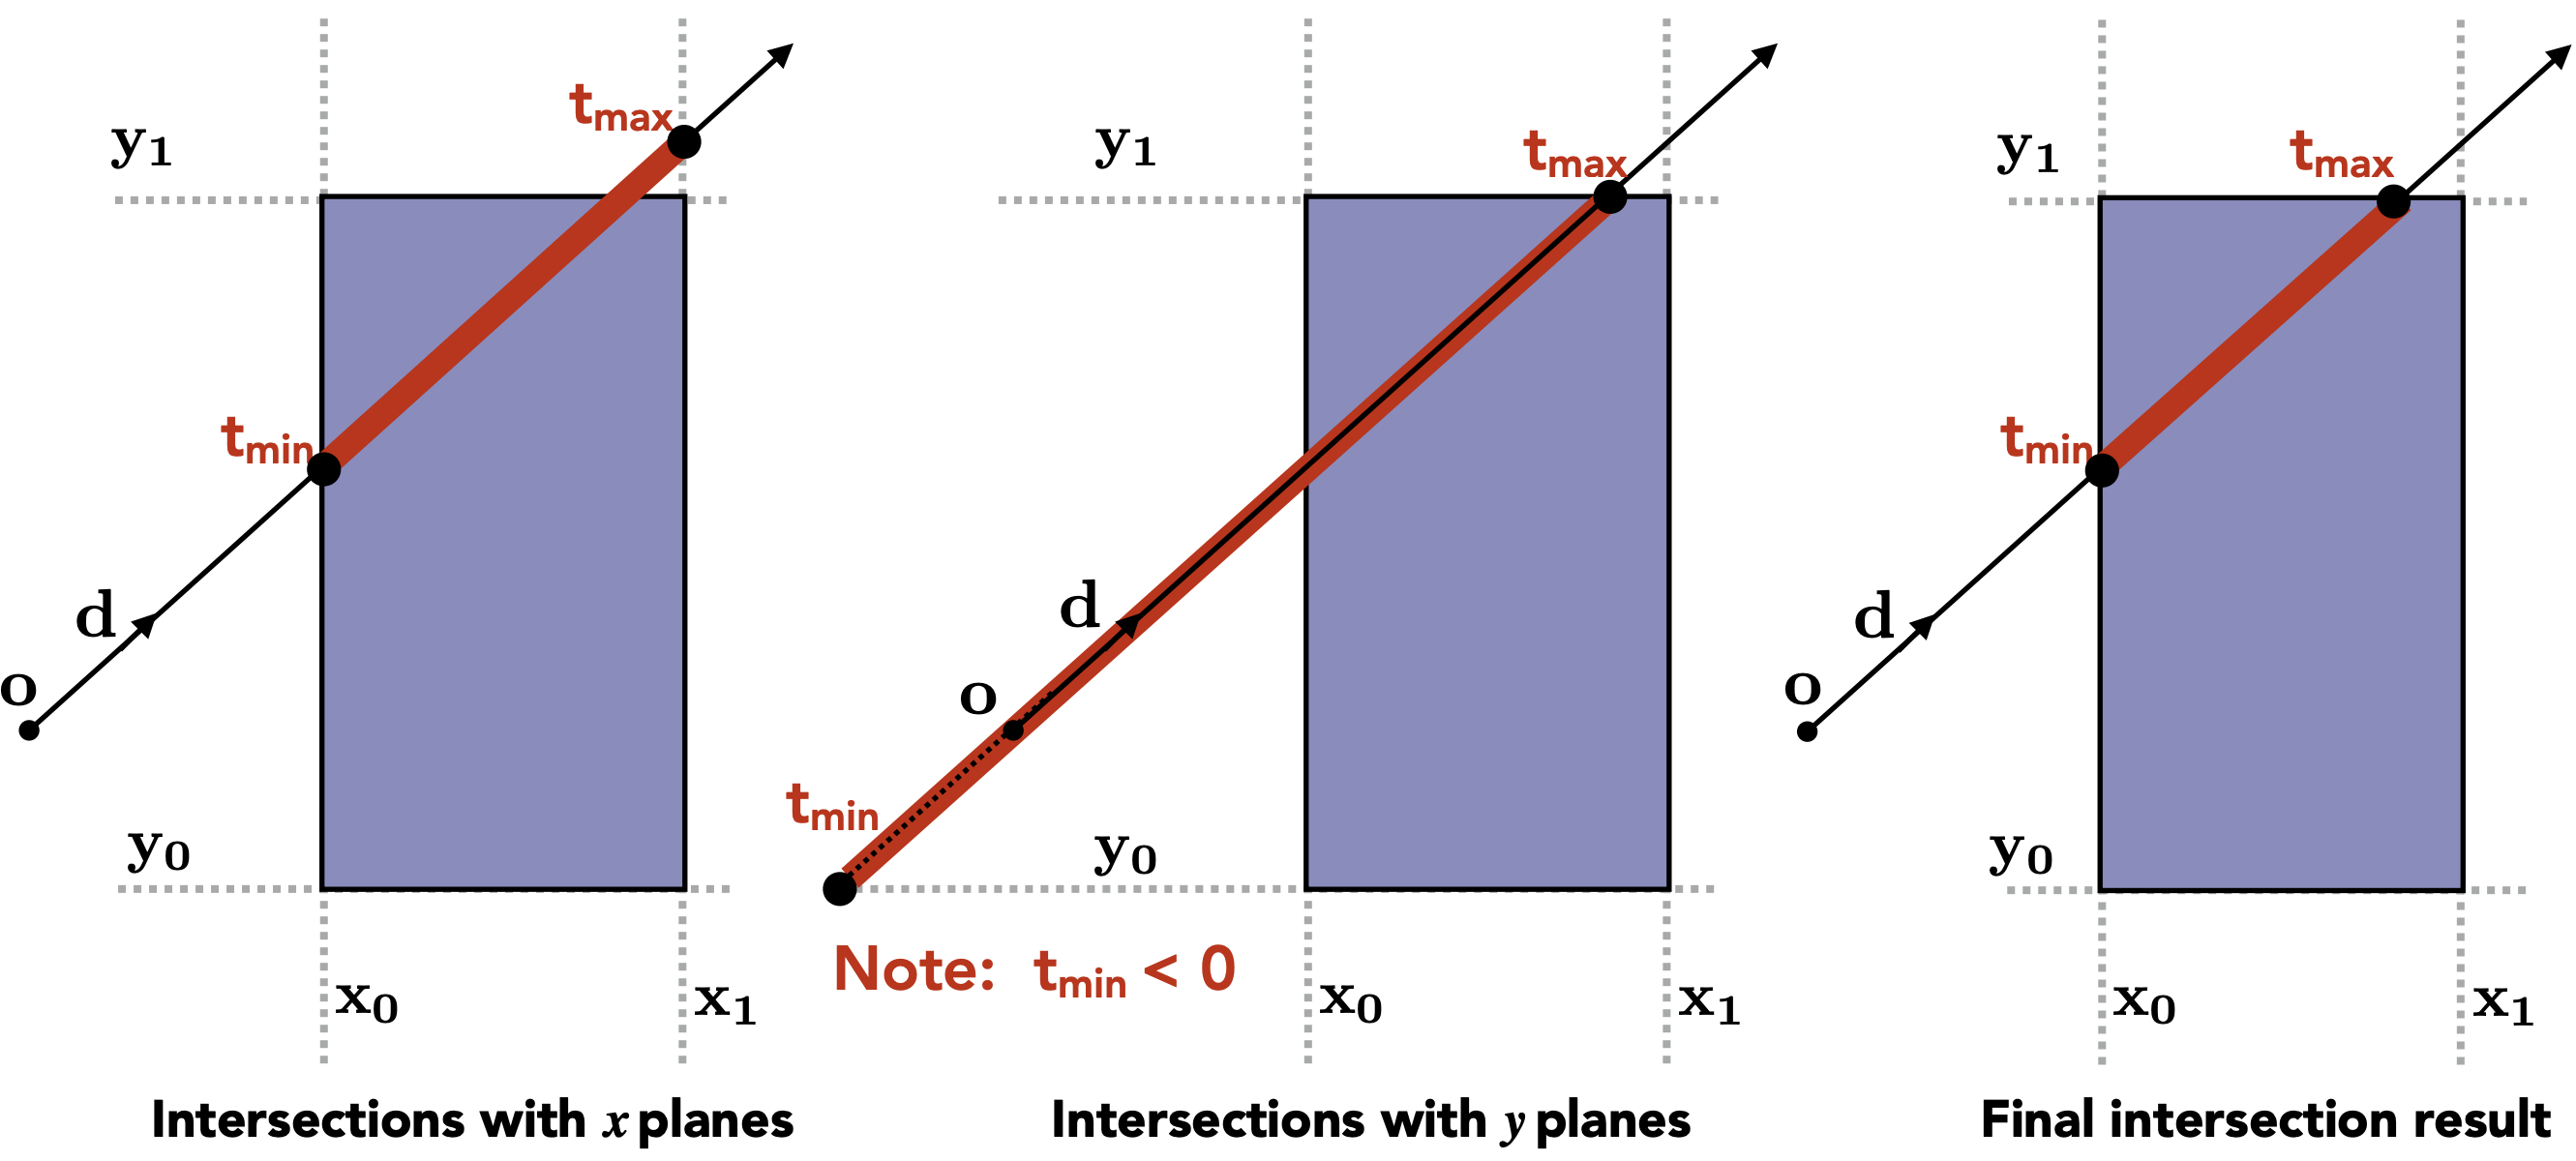
\includegraphics[scale=.25]{baoweitiji.png}
	\caption{包围体积中交点的计算}
	\label{fig:bwtj}
\end{figure}

我们求出光线在x平面上的两个交点以及y平面上的两个交点, 那么最终光线在包围盒内部的部分是这些交点区间的交集. 我们可以认为: 
\begin{itemize}
	\item 光线进入到三个面中, 才可以进入到包围盒; 
	\item 光线离开任意一个面, 就会离开包围盒. 
\end{itemize}
我们对三对面分别求出进入时间$t_{min}$和离开时间$t_{max}$, 那么最终对于包围盒来说进入时间$t_{enter}$是所有进入时间的最大值, 离开时间$t_{exit}$是所有离开时间的最小值. 如果进入时间小于离开时间, 那么我们认为光线和盒子有交点. 

对于时间出现负值的情况, 我们进行以下讨论: 
\begin{itemize}
	\item 如果离开时间$t_{exit}<0$, 那么盒子在光线的背后, 不会产生交点; 
	\item 如果进入时间$t_{enter} < 0$, 那么光线的起点在盒子的里面. 
\end{itemize}

光线和盒子有交点, 当且仅当 (iff) $t_{enter}<t_{exit}, t_{exit}\geq 0$.
我们可以利用三角形相似性求出对应的$t$值. 
\begin{figure}[H]
	\centering
	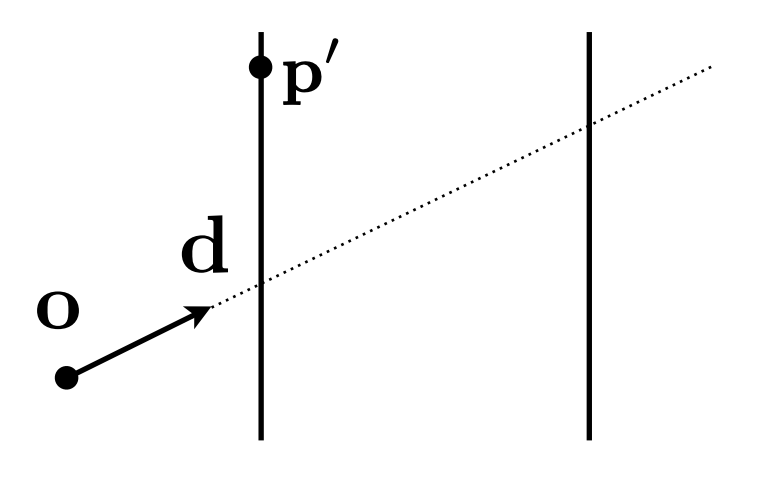
\includegraphics[scale=.25]{AABB.png}
	\caption{AABB中$t$值的计算}
	\label{fig:aabb}
\end{figure}
$t$值可以表示为: 
\begin{equation}
	t=\frac{p'_x-o_x}{d_x}
\end{equation}

\subsection{空间划分}
为了可以加速光线和物体求交点, 我们可以使用网格将原本比较大的包围盒进行划分. 我们进行网格划分分为以下几个步骤: 
\begin{enumerate}
	\item 找到场景中的包围盒; 
	\item 将包围盒划分成一个一个小格子; 
	\item 存储哪些小格子中包含物体 (我们认为物体都是非实心的面, 只记录包含面的小格子, 物体内部不包含面的小格子不计入) ; 
	\item 判断光线是否和格子相交, 如果光线和某个格子相交并且这个格子中包含物体, 那么我们需要与格子中的物体求光线的交点 (这里有两个假设: 1.判断光线和格子是否相交是很快的; 2.我们可以使用计算机图形学中画直线的方法来判断哪些格子是会相交的. ) . 
\end{enumerate}
\begin{figure}[H]
	\centering
	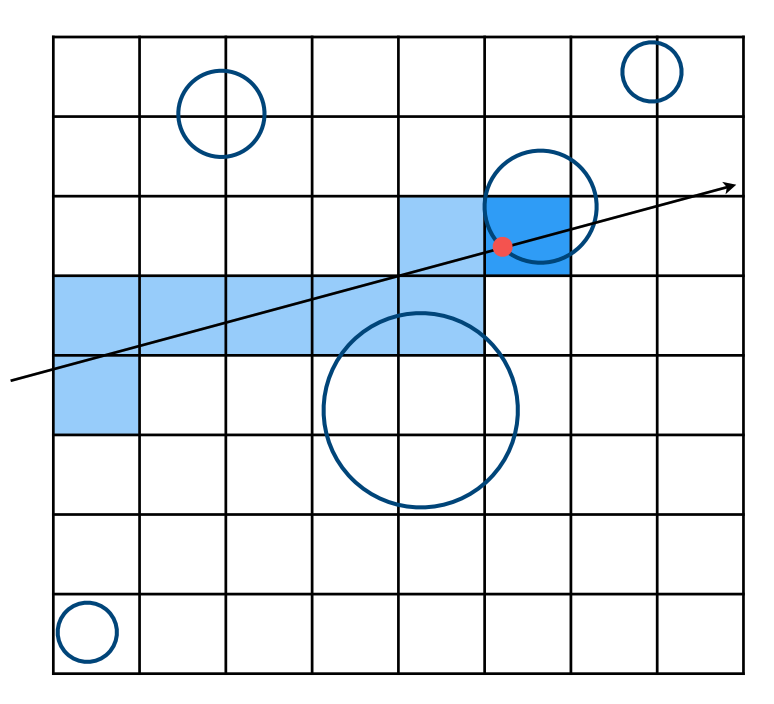
\includegraphics[scale=.15]{wanggehuafen.png}
	\caption{网格划分}
	\label{fig:wghf}
\end{figure}
一般来说, 格子的划分不可以太稀疏也不可以太稠密, 需要对格子的量进行控制. 这种划分方式对于物体分布均匀的场景比较合适. 对于物体分布稀疏的场景需要多次和格子进行相交判断, 这种方法相对不合适. 

我们会使用其他空间划分方法, 包括八叉树 (Oct-Tree) , KD树 (KD-Tree) 以及BSP树 (BSP-Tree) . 
\begin{figure}[H]
	\centering
	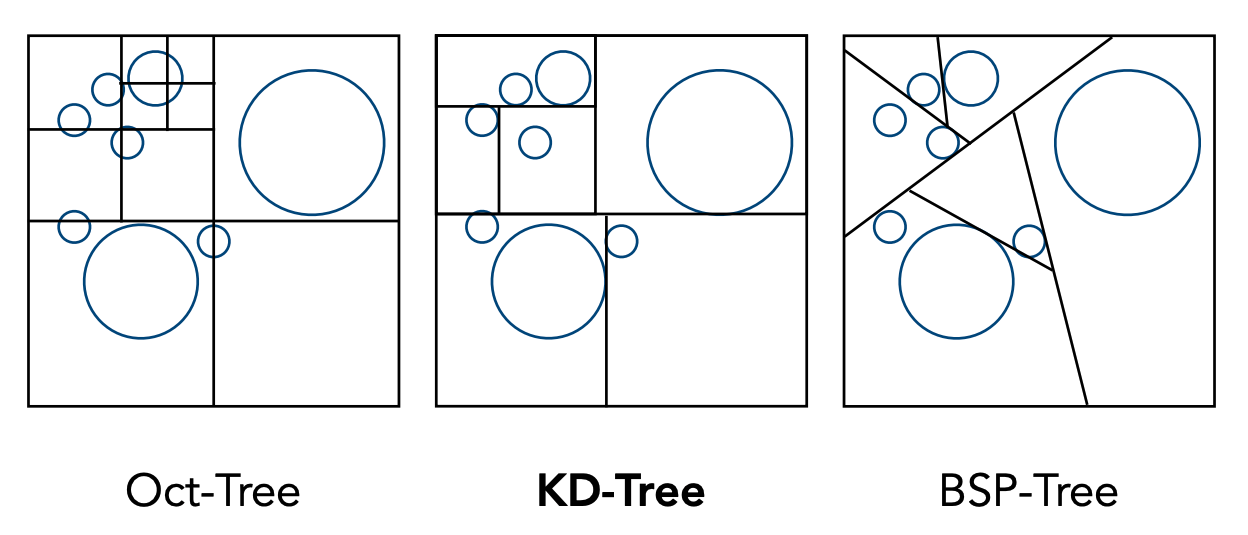
\includegraphics[scale=.15]{kongjianhuafen.png}
	\caption{空间划分}
	\label{fig:kjhf}
\end{figure}
\begin{itemize}
	\item \textbf{八叉树 (Oct-Tree) }, 将一个包围盒切成八块 (图中是二维情况, 只有4块) . 对于每一个小格子我们会继续进行划分直到小格子中没有物体或者物体的数量比较少; 
	\item \textbf{KD树 (KD-Tree) }, 每一次都进行一次水平划分或者竖直划分, 将包围盒分成两部分. 可以形成一个二叉树的存储结构. 水平划分和竖直划分交替进行, 保证划分的空间是均匀的; 
	\item \textbf{BSP树 (BSP-Tree) }, 每一次选择一个方向进行一次划分, 并不是沿着轴平行方向划分. 
\end{itemize}
三种划分方法, KD树更常用并且使用起来比较方便, 可以用二叉树来存储. 在每一个二叉树节点中, 我们都要储存以下信息: 
\begin{itemize}
	\item 如果是非叶子结点, 需要存储划分轴, 划分的位置以及孩子节点的指针; 
	\item 如果是叶子结点, 需要存储格子中包含的物体. 
\end{itemize}

实际划分出的盒子均在叶子结点上. 

\begin{figure}[H]
	\centering
	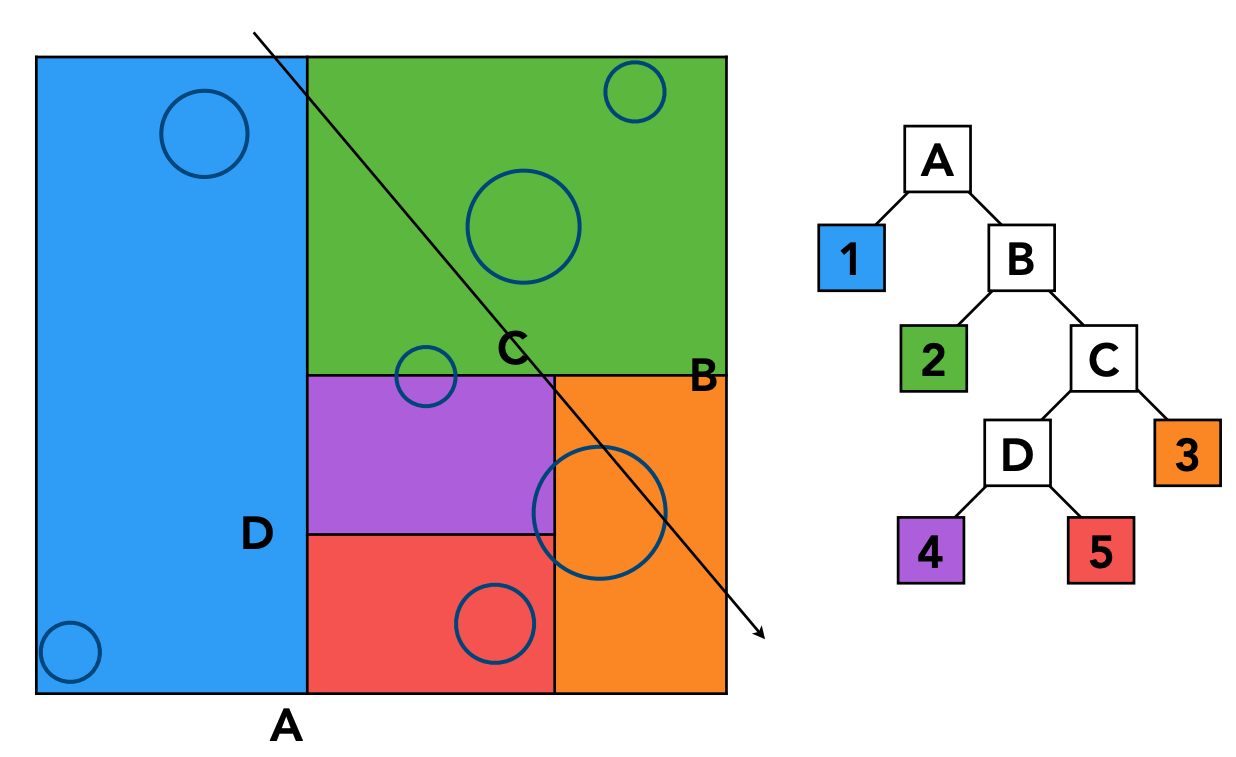
\includegraphics[scale=.15]{kongjianhuafenjisuan.png}
	\caption{空间划分后计算光线和物体的交点}
	\label{fig:kjhfjs}
\end{figure}
我们通过类似于二分查找的方式计算交点: 
\begin{itemize}
	\item 如果光线和一个节点有交点, 那么它和它的子节点也有交点; 
	\item 如果光线和叶子结点有交点, 那么它需要和格子内的所有物体求交点. 
\end{itemize}
这种方法存在两个问题, 首先, 格子和一个三角形面是否相交的判断比较复杂. 第二, 一个物体可能会在多个不同的格子中, 需要多次存储. 因此我们会使用更常用的物体划分的方式. 

\subsection{物体划分}
\textbf{物体划分 (Bounding Volume Hierarchy, BVH) }的主要思想是对物体进行进行划分, 并重新计算包围盒. BVH中, 每一个物体只属于一个包围盒. BVH的划分主要分为三步: 
\begin{enumerate}
	\item 划分包围盒; 
	\item 递归的将包围盒划分为两部分; 
	\item 当叶子结点的三角形面数量足够少的时候, 停止划分. 
\end{enumerate}
当我们进行划分的时候, 也有不同的划分技巧: 
\begin{itemize}
	\item 沿着最长的轴划分为两半 (让长轴变短, 分割更加均匀) ; 
	\item 取中间的物体进行划分, 可以保证两边三角形数量差不多 (找到第k个物体的算法可以在$o(n)$的时间内解决, 被称作快速选择算法) ; 
	\item 当包围盒中的物体数量小于一定数量的时候停止划分. 
\end{itemize}
使用伪代码可以写成如下形式: 
\begin{lstlisting}[
	caption={BVH伪代码},
	language=c]
	Intersect(Ray ray, BVH node) {
		if (ray misses node.bbox) return;
		
		if (node is a leaf node)
			test intersection with all objs;
			return closest intersection;
		
		hit1 = Intersect(ray, node.child1);
		hit2 = Intersect(ray, node.child2);
		return the closer of hit1, hit2;
	}
\end{lstlisting}
这是一个递归算法. 

\chapter{辐射度量学}
不论是光栅化还是光线追踪, 都是对我们现实光照的近似表示. 因此我们提出辐射度量学通过精准的物理定义模拟光照环境, 使用更真实的方式进行光线追踪. 辐射度量学描述了Radiant flux, intensity, irraddiance以及radiance. 

\section{Radiant Energy and Flux}
\textbf{Radiant Energy} 指的是电磁辐射的能量. 用符号$\mathbf{Q}$表示, 单位是焦耳$\mathbf{J}$.

\textbf{Radiant Flux (Power) } 指的是单位时间的能量. $\Phi=\frac{dQ}{dt}$, 单位是瓦特$\mathbf{W}$,也可以用单位$\mathbf{lm}$叫做流明 (lumen) . 是单位时间通过一个平面光照的量. 

\section{Radiant Intensity}
\textbf{Radiant Intensity}指的是光源在单位立体角上的能量. 数学定义为: 
\begin{equation}
	I(\omega)=\frac{d\Phi}{d\omega}
\end{equation} 单位为$\mathbf{W}/\mathbf{sr}$或者坎德拉$\mathbf{candela}=\mathbf{cd}=\frac{\mathbf{lm}}{\mathbf{sr}}$.

\subsection{单位立体角}
在二维平面上, 我们使用弧度制定义角度, 定义为角度对应圆上的弧长除以半径: 
\begin{equation}
	\theta = \frac{l}{r}
\end{equation} 单位是$\mathbf{rad}$.整圆对应的角度为$2\pi\ \mathbf{rad}$.

我们定义立体角为角度在球上对应的面积除以半径的平方: 
\begin{equation}
	\omega=\frac{A}{r^2}
\end{equation} 单位是$\mathbf{sr}$, 整球对应的立体角为$4\pi\ \mathbf{sr}$.

接下来我们推出\textbf{单位立体角 (Differential Solid Angles) }的公式: 
\begin{figure}[H]
	\centering
	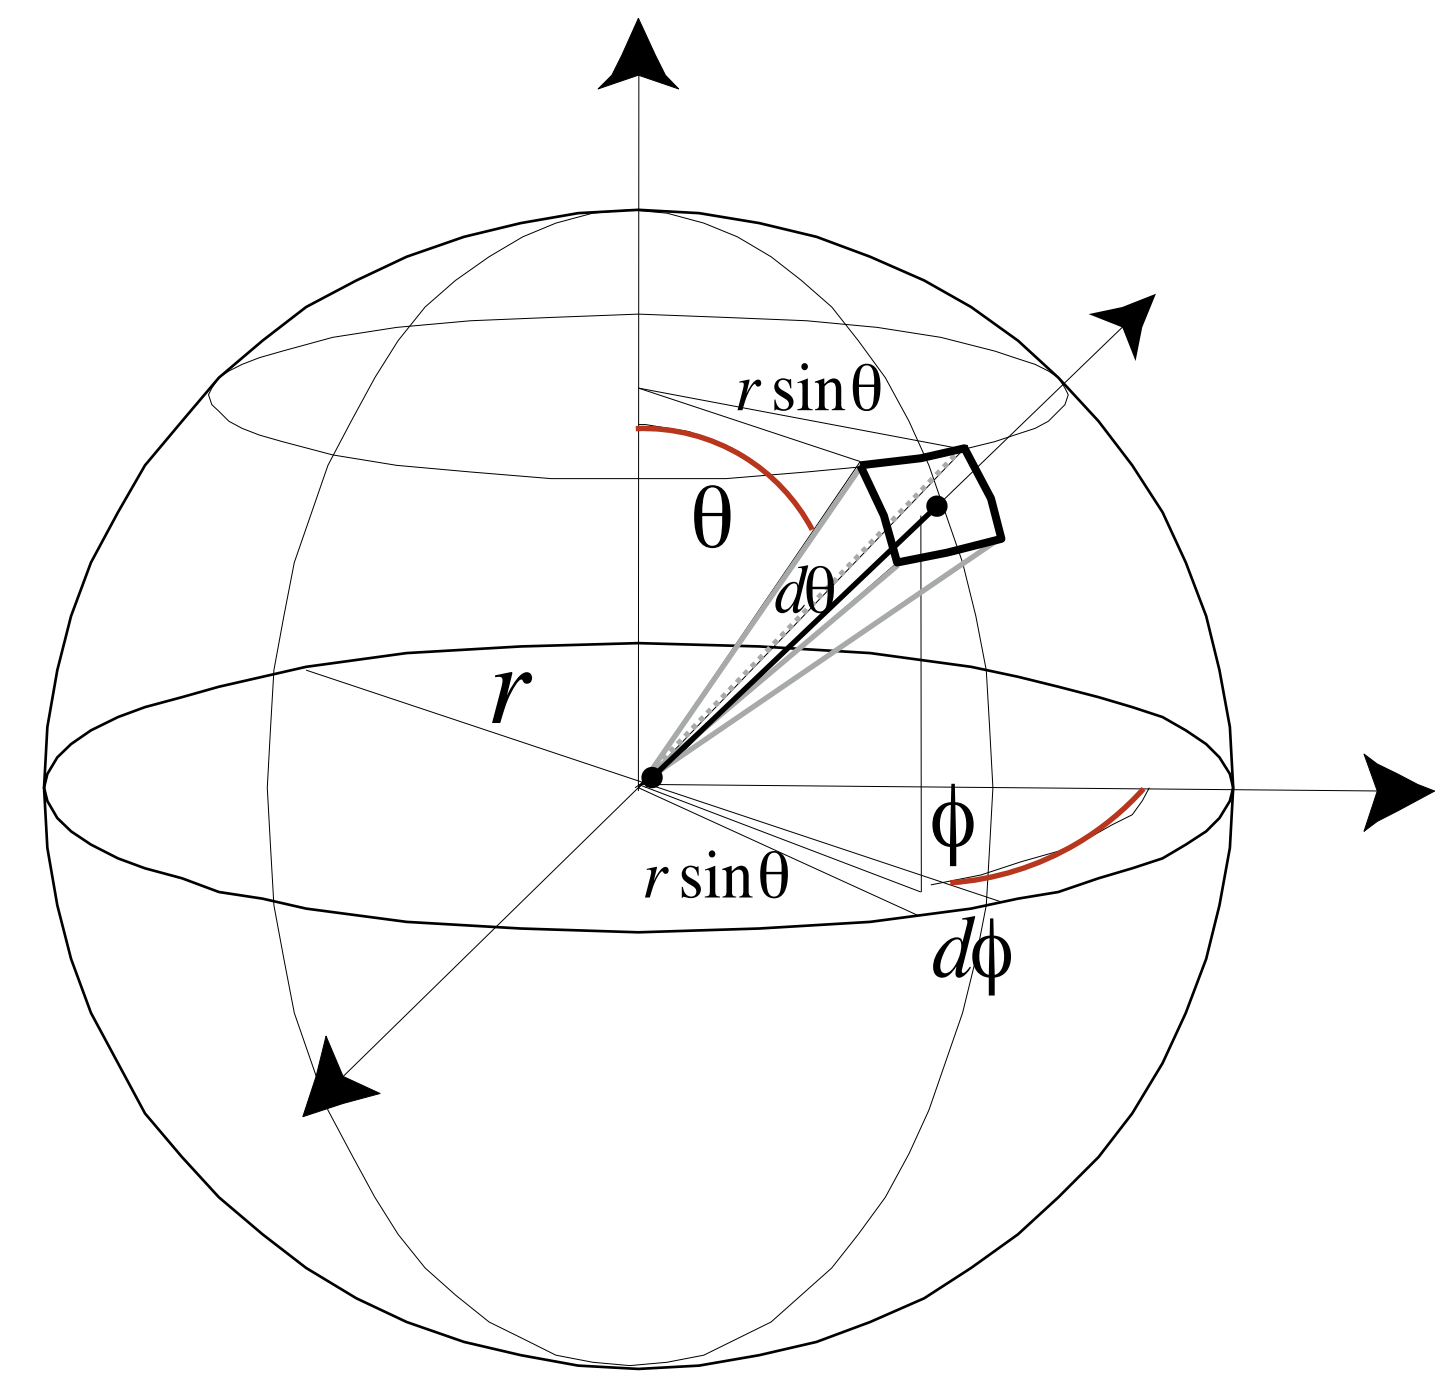
\includegraphics[scale=.25]{danweilitijiao.png}
	\caption{单位立体角推理}
	\label{fig:dwltj}
\end{figure}

\begin{equation}
\begin{split}
	dA=(rd\theta)(r\sin \theta d \phi)=r^2\sin\theta d\theta d\phi \\
	d\omega=\frac{dA}{r^2}=\sin\theta d\theta d\phi
\end{split}
\end{equation}

我们使用积分进行验证, 对整个球面的单位立体角进行积分: 
\begin{equation}
	\begin{split}
		\Omega=\int_{S^2}d\omega=\int_{0}^{2\pi}\int_{0}^{\pi}\sin\theta d\theta d\phi = 4\pi
	\end{split}
\end{equation}

因此, 对于一个均匀发光的光源, $I=\frac{\Phi}{4\pi}$. 

\section{Irradiance}

\textbf{Irradiance}指的是单位面积上所接收到的能量. 定义为: 
\begin{equation}
	E(x)=\frac{d\Phi(x)}{dA\cos\theta}
\end{equation} 单位是$\mathbf{W}/\mathbf{m}^2$或者$\mathbf{lux}=\frac{\mathbf{lm}}{\mathbf{m}^2}$.接收到的能量应当是和平面垂直的光线带来的能量. 如果光线和平面不垂直, 我们需要将光线投影到平面的法线上, $\theta$是光线和平面法线的夹角. 

我们回顾对于光能量衰减的理解, 我们在Blinn-Phong模型中认为, 点光源能量和距离成平方反比的关系. 我们使用Irradiance来解释这个现象. 我们认为任何一个球面上的Intensity不会发生衰减, 之所以光的能量会发生衰减, 正是因为相同的立体角下对应的球面面积增加, 使得Irradiance发生变化. 因此, 点光源在某一个球面上的Irradiance和距离依然是平方反比关系. 

\section{Radiance}
\textbf{Radiance}描述了光线的属性, 它代表单位立体角单位面积上的能量. 
\begin{figure}[H]
	\centering
	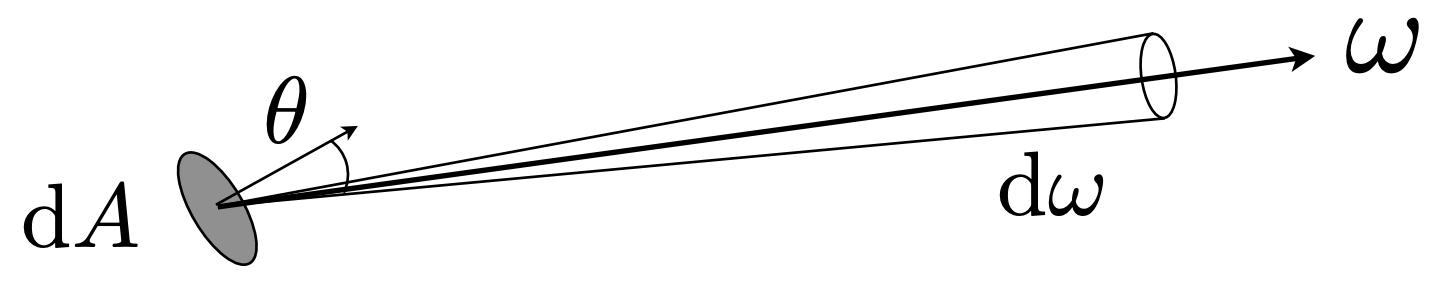
\includegraphics[scale=.25]{radiance.png}
	\caption{Radiance的计算}
	\label{fig:radiance}
\end{figure}

\begin{equation}
	L(p,\omega)=\frac{d^2\Phi(p,\omega)}{d\omega dA\cos\theta}
\end{equation} 单位是$\mathbf{W}/(\mathbf{sr}\cdot \mathbf{m}^2)$或者$\mathbf{nit}=\frac{\mathbf{lm}}{\mathbf{sr}\ \mathbf{m}^2}=\frac{\mathbf{cd}}{\mathbf{m}^2}$.我们可以从两个方面来理解Radiance. 从入射角度来说, 我们认为Radiance是单位立体角下的Irradiance: 
\begin{equation}
	L(p,\omega)=\frac{dE(p)}{d\omega \cos\theta}
\end{equation}

从出射的角度来说, 我们认为Radiance是单位面积下的Intensity: 
\begin{equation}
		L(p,\omega)=\frac{dI(p,\omega)}{dA \cos\theta}
\end{equation}

\section{Irradiance vs. Radiance}
\textbf{Irradiance}: 面积$dA$接收的所有能量

\textbf{Radiance}: 面积$dA$从指定\enquote{方向}$d\omega$接收到的能量

Irradiance也可以表示为Radiance在所有角度上的积分: 
\begin{equation}
	\begin{split}
		dE(p,\omega)=L_i(p,\omega)\cos\theta d\omega\\
		E(p)=\int_{H^2}L_i(p,\omega)\cos\theta d\omega
	\end{split}
\end{equation}我们只对上半球做积分, 我们认为和法线方向相反的光线对这一点没有贡献. 

\begin{figure}[H]
	\centering
	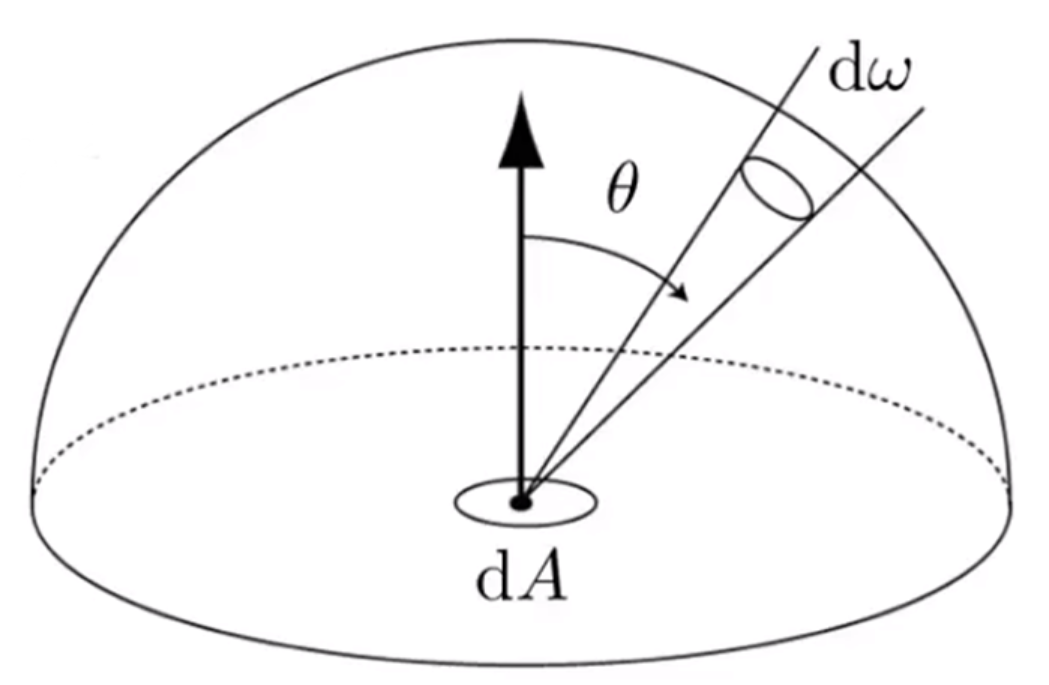
\includegraphics[scale=.4]{vs.png}
	\caption{Irradiance vs. Radiance}
	\label{fig:vs}
\end{figure}

\section{双向反射分布函数}
\textbf{双向反射分布函数 (Bidirectional Reflectance Distribution Fuction, BRDF) }定义了一个函数来表示从某一个角度入射的光线在某一个角度上会有多少能量被反射出去. 我们将反射的过程理解为两步: 第一步, 光线入射物体得到了一部分能量; 第二步, 物体将得到的能量再一次射出去. 

\begin{figure}[H]
	\centering
	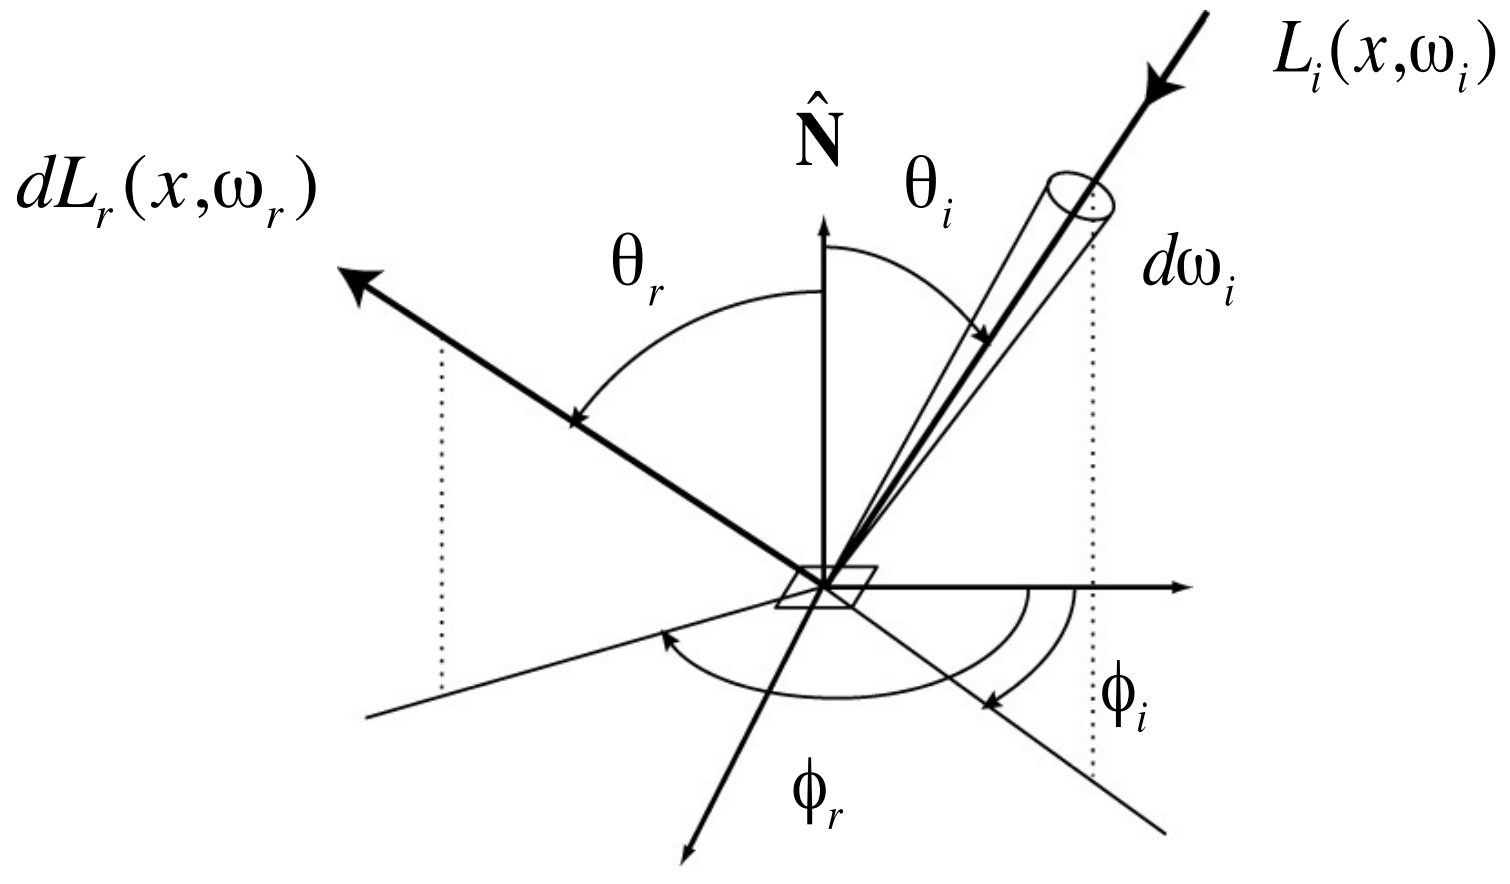
\includegraphics[scale=.35]{brdf.png}
	\caption{BRDF的定义}
	\label{fig:brdf}
\end{figure}

因此, 我们定义双向反射分布函数为: 
\begin{equation}
	f_r(\omega_i\rightarrow \omega_r)=\frac{dL_r(\omega_r)}{dE_i(\omega_i)}=\frac{dL_r(\omega_r)}{L_i(\omega_i)\cos\theta_i d\omega_i}[\frac{1}{sr}]
\end{equation}

那么, 对于某一个出射方向, 对应的能量应该是所有入射角度的光线反射结果的叠加: 
\begin{equation}
	L_r(p,\omega_r)=\int_{H^2}f_r(\omega_i\rightarrow \omega_r)L_i(p,\omega_i)\cos\theta_id\omega_i
\end{equation}

一个物体除了会反射来自其他物体的光线之外, 这个物体还有可能会自发光. 因此, 我们定义\textbf{渲染函数}为: 
\begin{equation}
	L_o(p,\omega_o)=L_e(p,\omega_o)+\int_{\Omega^+}L_i(p,\omega_i)f_r(p,\omega_i,\omega_o)(n\cdot \omega_i)d\omega_i
\end{equation}渲染函数包含两部分, 一部分是物体自发光, 另一部分是反射光. 在这里我们使用点乘代替$\cos\theta$计算. 我们的积分区域只在上半球, 法线反方向光线对于平面没有贡献. 

我们再一次理解这个公式, 我们可以认为$L_i$包含其他点光源, 面光源以及其他物体二次反射光线. 最终结果我们使用积分的方式进行叠加. 那么这个公式可以简写为: 
\begin{equation}
	I(u)=e(u)+\int I(v)K(d,v)dv
\end{equation} 我们可以通过矩阵再一次简化公式为: 
\begin{equation}
	l=E+KL
\end{equation}
通过求解矩阵我们可以得到: 
\begin{equation}
	L=(I-K)^{-1}E
\end{equation}

我们可以将矩阵进行展开, 可以得到: 
\begin{equation}
	\begin{split}
		L&=(1+K+K^2+K^3+\dots)E\\
		&=E+KE+K^2E+K^3E+\dots
	\end{split}
\end{equation}
每一项分别代表的是: 物体直接发出的光, 光源经过一次反射的光, 光源经过两次反射得到的间接光照, ……

\section{全局光照}
全局光照指的是直接光照以及间接光照的集合. 光栅化处理的是0次项和1次项的部分, 对于高阶项比较难处理. 随着我们不断叠加不同反射次数的结果, 图片会收敛到一个亮度, 不会一直变亮.

\chapter{蒙特卡洛路径追踪}

我们在上一节得到了渲染函数为
\begin{equation}
	L_o(p,\omega_o)=L_e(p,\omega_o)+\int_{\Omega^+}L_i(p,\omega_i)f_r(p,\omega_i,\omega_o)(n\cdot \omega_i)d\omega_i
\end{equation}
本节我们将通过数学工具求解这个函数并写成算法的形式来实现路径追踪. 

\section{蒙特卡洛积分}

对于任意一个函数, 不论是可以简单表达成解析式的还是不能轻松表达为解析式的函数, 我们都希望求出其定积分的结果. 在高等数学中我们使用\textbf{黎曼积分}求解. 也就是我们将曲线下的面积近似成一系列的小长方形的和. 当小长方形越多时, 得到的结果越相近. 

蒙特卡洛积分是通过多次随机采样并将采样对应的结果除以其概率密度的平均值作为积分结果. 也就是说对于一个采样概率分布$X_i\sim p(x)$, 蒙特卡洛积分为
\begin{equation}
	\int_a^b f(x) = F_N=\frac{1}{N}\sum_{i=1}^N\frac{f(X_i)}{p(X_i)}
\end{equation}

我们假设采样的概率分布是均匀分布, 也就是说$X_i\sim p(x)=\frac{1}{b-a}$, 那么蒙特卡洛积分可以表示为
\begin{equation}
	\int_a^b f(x) = F_N=\frac{b-a}{N}\sum_{i=1}^Nf(X_i)
\end{equation}

蒙特卡洛积分对于任何一种采样分布都是成立的. 只要进行采样就可以得到对应的积分. 使用蒙特卡洛积分要注意两点: 
\begin{enumerate}
	\item 采样的次数越多, 得到的结果越准确; 
	\item 采样必须在积分域上进行采样. 
\end{enumerate}

\section{路径追踪}
在之前的课程中我们介绍了Whitted-Style光线追踪, 但是这种追踪方式具有其极限性. Whitted-Style光线追踪仅计算光线的镜面反射, 因此对于某些弱于镜面反射的光线反射现象 (这里称作Glossy) 不能进行很好的表示. 因此我们选择使用渲染方程得到更加准确的求解. 

对于渲染函数我们有两个问题需要解决: 
\begin{enumerate}
	\item 我们需要求解积分项; 
	\item 这是一个递归的函数. 
\end{enumerate}

\subsection{积分求解}

使用蒙特卡洛积分求解积分项. 在这里我们限定仅计算来自光源的光线, 如果是来自其他物体的光线, 这里我们看作0.

我们和蒙塔卡洛积分进行对照, 发现$f(x)$对应的是$L_i(p,\omega_i)f_r(p,\omega_i,\omega_o)(n\cdot \omega_i)$. 积分域是$\omega_i$, $\omega_i$在上半球均匀分布采样的概率密度为$\frac{1}{2\pi}$. 

因此渲染函数的积分项可以写成: 
\begin{equation}
	\begin{split}
		L_o(p,\omega_o)&=\int_{\Omega^+}L_i(p,\omega_i)f_r(p,\omega_i,\omega_o)(n\cdot \omega_i)d\omega_i\\
		&\approx \frac{1}{N}\sum_{i=1}^{N}\frac{L_i(p,\omega_i)f_r(p,\omega_i,\omega_o)(n\cdot \omega_i)}{p(\omega_i)}
	\end{split}
\end{equation}

这样的过程我们可以写成伪代码的形式: 
\begin{lstlisting}[caption=渲染函数积分项对光源光线求解伪代码]
shade(p, wo)
	Randomly choose N directions wi~pdf
	Lo = 0.0
	For each wi
		Trace a ray r(p, wi)
		If ray r hit the light
			Lo += (1 / N) * L_i * f_r * cosine / pdf(wi)
	Return Lo
\end{lstlisting}

对于间接光照, 对于下图中的P点, 如果我们想要求出来自Q点的光线, 我们可以看作我们从P点看向Q点来自光源的光线反射得到的结果. 那么以上的伪代码我们可以改写为递归的形式: 


\begin{figure}[H]
	\centering
	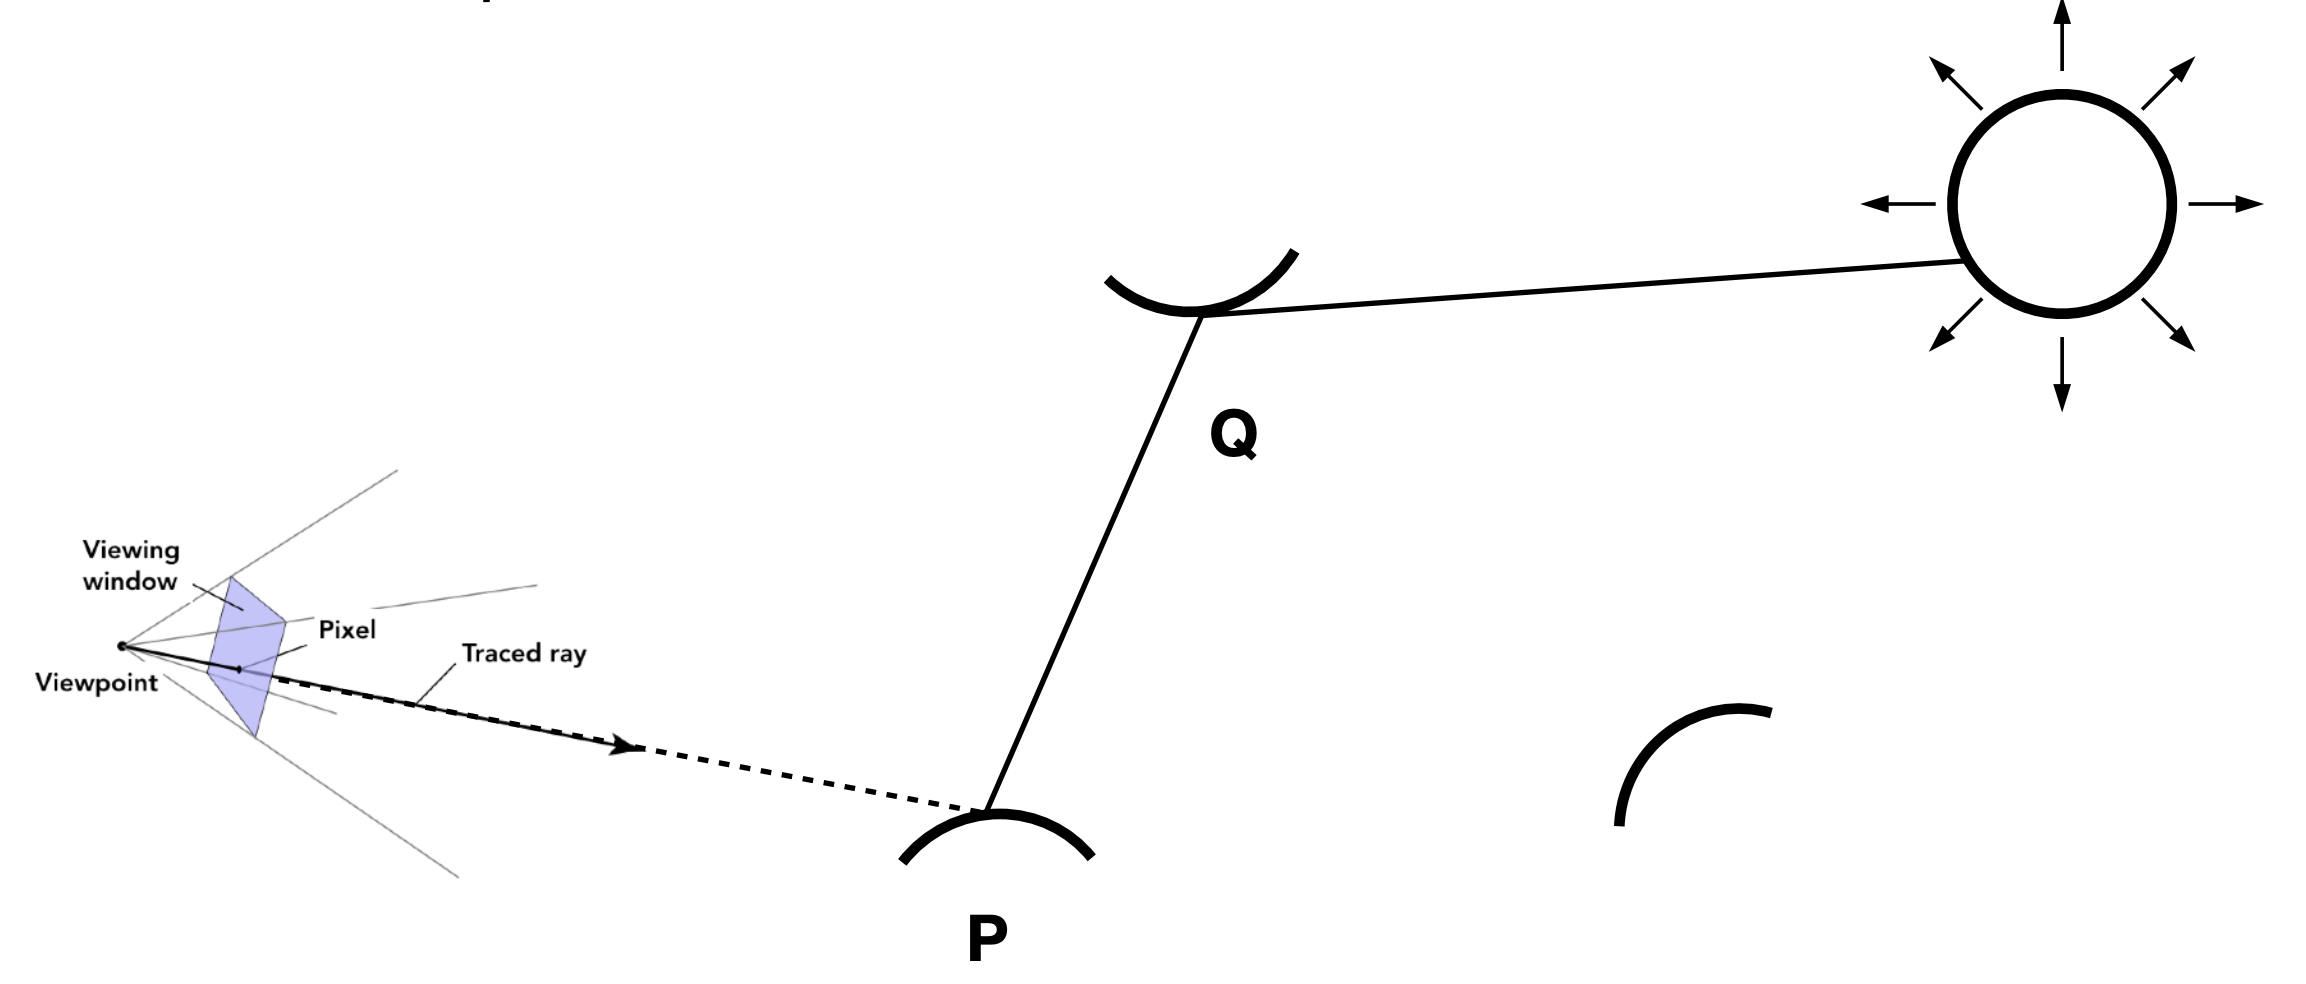
\includegraphics[scale=.25]{jianjieguangzhao.png}
	\caption{间接光照的递归求解}
	\label{fig:jjgz}
\end{figure}

\begin{lstlisting}[caption=渲染函数积分项的递归求解伪代码]
shade(p, wo)
	Randomly choose N directions wi~pdf
	Lo = 0.0
	For each wi
		Trace a ray r(p, wi)
		If ray r hit the light
			Lo += (1 / N) * L_i * f_r * cosine / pdf(wi)
		Else If ray r hit an object at q
			Lo += (1 / N) * shade(q, -wi) * f_r * cosine / pdf(wi)
	Return Lo
\end{lstlisting}

\subsection{算法优化}

\subsubsection{指数爆炸问题}

如果我们采样$N$次, 那么在经过$r$次反射后, 光线的数目可以达到$N^r$条, 会使计算量大大增加. 当且仅当$N=1$的时候, 不会产生指数爆炸问题. 此时我们转变方法, 在计算积分的时候我们仅计1次, 但是我们会在同一个像素中多次采样. 也就是说, 同一个像素上应该有多条光线通过, 我们对这些光线分别计算渲染函数后求平均就是这一像素的结果. 这个方法就是\textbf{路径追踪 (Path Tracing) }. 

\begin{lstlisting}[caption=渲染函数解决指数爆炸伪代码]
ray_generation(camPos, pixel)
	Uniformly choose N sample positions within the pixel
	pixel_radiance = 0.0
	For each sample in the pixel
		Shoot a ray r(camPos, cam_to_sample)
		If ray r hit the scene at p
			pixel_radiance += 1 / N * shade(p, sample_to_cam)
	Return pixel_radiance
\end{lstlisting}

\subsubsection{递归的停止问题}
我们的算法使用到了递归的方式. 但是我们的算法没有递归的结束条件. 因此我们需要引入一种方式结束递归. 我们引入俄罗斯轮盘赌 (RR) 的方式. 每一次光线都有$p$的概率能够反射出来. 如果说光线可以反射, 那么继续计算. 反之直接返回0.那么伪代码的形式是: 

\begin{lstlisting}[caption=包含递归停止条件的渲染函数伪代码]
shade(p, wo)
	Manually specify a probability P_RR
	Randomly select ksi in a uniform dist. in [0, 1]
	If (ksi > P_RR) return 0.0;
	 
	Randomly choose ONE directions wi~pdf
	Trace a ray r(p, wi)
	If ray r hit the light
		Return (1 / N) * L_i * f_r * cosine / pdf(wi) / P_RR
	Else If ray r hit an object at q
		Return (1 / N) * shade(q, -wi) * f_r * cosine / pdf(wi) / P_RR
\end{lstlisting}

我们返回的结果最终都会除以概率$p$, 这样子, 这一点得到结果的期望值和原来一样. 每一条光线反射次数的期望值是$\frac{p}{(1-p)^2}$.

\subsubsection{均匀分布并非最优解}

对于同一个点来说, 光源面积大, 那么我们使用较少的光线就可以接触到光源. 但是如果光源面积太小, 我们必须使用较多的光线才可以和光源发生接触. 那么对于小光源计算量会上升. 因此我们希望使用其他的概率分布进行采样, 使得采样得到的光线基本上都在光源上. 

我们的解决方案是在光源上进行均匀分布的采样, 这样子所有的光线一定都是来自于光源的. 

\begin{figure}[H]
	\centering
	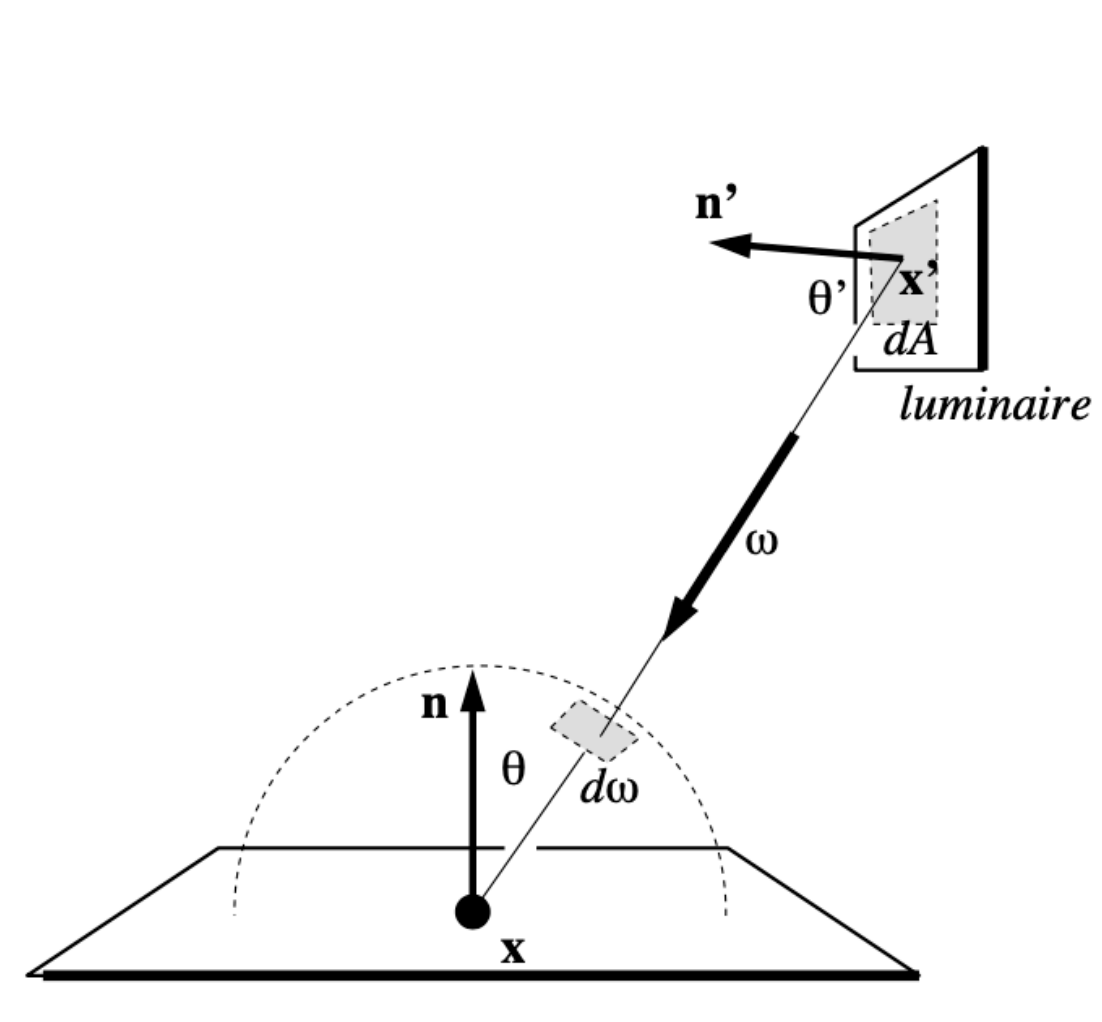
\includegraphics[scale=.25]{samplelight.png}
	\caption{从光源进行采样}
	\label{fig:samplelight}
\end{figure}

我们光源$A$上进行采样, 那么概率密度应该是$\frac{1}{A}$. 但是蒙特卡洛积分的采样必须在积分域上. 此时积分域发生了变换, 我们需要找到$d\omega$和$dA$之间的关系. $d\omega$是$dA$在对应单位球上的投影, 因此
\begin{equation}
	d\omega = \frac{dA\cos\theta'}{||x'-x||^2}
\end{equation}

那么积分式就可以改变为: 
\begin{equation}
	\begin{split}
		L_o(p,\omega_o)&=\int_{\Omega^+}L_i(p,\omega_i)f_r(p,\omega_i,\omega_o)\cos\theta d\omega_i\\
		&=\int_AL_i(p,\omega_i)f_r(p,\omega_i,\omega_o)\frac{\cos\theta\cos\theta'}{||x'-x||^2}dA
	\end{split}
\end{equation}

此时, 我们需要更改一下之前RR的策略. 对于直接光照, 不使用RR; 对于间接光照使用RR. 这样我们就把问题分为了两部分——直接光照和间接光照. 

\begin{lstlisting}[caption=采用光源上均匀分布渲染函数伪代码]
shade(p, wo)
	# Contribute from the light source
	Uniformly sample the light at x' (pdf_light = 1 / A)
	L_dir = L_i * f_r * cos(theta) * cos(theta') / |x' - p| ^ 2 / pdf_light
	
	# Contribute from other reflectors
	L_indir = 0.0
	Test Rassian Roulette with probability P_RR
	Uniformly sample the hemisphere toward wi (pdf_hemi = 1 / 2pi)
	Trace a ray r(P, wi)
	If ray r hit a non-emitting object at q
		L_indir = shade (q, -wi) * f_r * cos(theta) / pdf_hemi / P_RR
	
	Return L_dir + L_indir
\end{lstlisting}

最后我们只需要对光源和反射点间有物体的情况进行判断即可, 

\begin{lstlisting}[caption=渲染函数伪代码]
	shade(p, wo)
	# Contribute from the light source
	L_dir = 0.0
	Uniformly sample the light at x' (pdf_light = 1 / A)
	Shoot a ray from p to x'
	If the ray is not blocked in the middle
		L_dir = L_i * f_r * cos(theta) * cos(theta') / |x' - p| ^ 2 / pdf_light
	
	# Contribute from other reflectors
	L_indir = 0.0
	Test Rassian Roulette with probability P_RR
	Uniformly sample the hemisphere toward wi (pdf_hemi = 1 / 2pi)
	Trace a ray r(P, wi)
	If ray r hit a non-emitting object at q
	L_indir = shade (q, -wi) * f_r * cos(theta) / pdf_hemi / P_RR
	
	Return L_dir + L_indir
\end{lstlisting}

这样我们就得到了最终路径追踪的算法. 

